\documentclass[coursework]{SCWorks}
\usepackage{preamble}

\chair{математической кибернетики и компьютерных наук}
\title{Исследование алгоритмов машинного обучения для классификации данных}
\course{1}
\group{151}
\napravlenie{09.03.04 --- Программная инженерия}
\author{Ахмеджановой Алины Рамилевны}
\date{2026}

\satitle{доцент, к.\,ф.-м.\,н.}

\chtitle{профессор, д.\,ф.-м.\,н.}


\secNumbering

\begin{document}

\maketitle
\tableofcontents

\intro

В современном мире задачи классификации данных являются одними из ключевых в области машинного обучения. В данной работе рассматривается применение методов машинного обучения для решения задачи классификации с использованием библиотеки \texttt{scikit-learn} \cite{henrick2017ml}.

\section{Теоретические основы}

\subsection{Метод опорных векторов}

Метод опорных векторов (SVM) — это алгоритм классификации, который строит гиперплоскость, разделяющую классы. Оптимальная гиперплоскость находится путем решения задачи оптимизации:

\begin{equation}
\min_{\mathbf{w}, b} \frac{1}{2} \|\mathbf{w}\|^2 + C \sum_{i=1}^{n} \max(0, 1 - y_i(\mathbf{w}^T \mathbf{x}_i + b))
\label{eq:svm}
\end{equation}

\subsection{Логистическая регрессия}

Логистическая регрессия использует сигмоидную функцию для предсказания вероятности принадлежности к классу:

\begin{equation}
P(y=1|\mathbf{x}) = \frac{1}{1 + e^{-(\mathbf{w}^T \mathbf{x} + b)}}
\label{eq:sigmoid}
\end{equation}

\subsection{Градиентный бустинг}

Градиентный бустинг строит ансамбль деревьев решений последовательно, где каждое следующее дерево исправляет ошибки предыдущих:

\begin{equation}
F_m(x) = F_{m-1}(x) + \gamma_m h_m(x)
\label{eq:gb}
\end{equation}

На рисунке~\ref{fig:svm_visualization} показана визуализация работы метода опорных векторов.

\begin{figure}[ht]
\centering
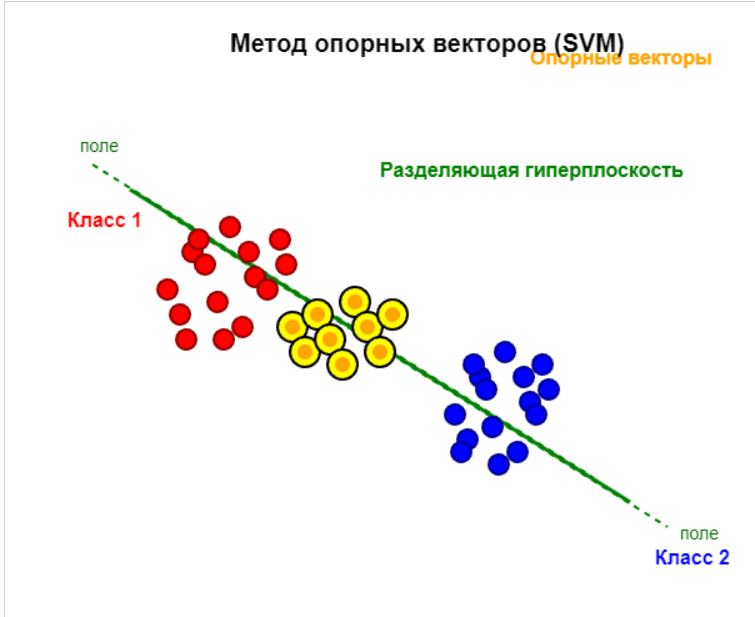
\includegraphics[width=0.8\textwidth]{figures/svm_visualization.png}
\caption{Визуализация метода опорных векторов}
\label{fig:svm_visualization}
\end{figure}

\section{Практическая реализация}

\subsection{Программный код на Python}

Полный исходный код программы находится в файле \texttt{code/ml_classification.py}. Ниже представлена реализация:

\lstinputlisting[language=Python, caption={Реализация на Python}, label=code:python]{code/ml_classification.py}

\subsection{Программный код на C++}

Альтернативная реализация на языке C++ представлена в файле \texttt{code/ml_classification.cpp}:

\lstinputlisting[language=C++, caption={Реализация на C++}, label=code:cpp]{code/ml_classification.cpp}

\section{Экспериментальные результаты}

В процессе обучения модели на наборе данных использовались различные гиперпараметры. На рисунке~\ref{fig:learning_curve} показана кривая обучения модели.

\begin{figure}[ht]
\centering
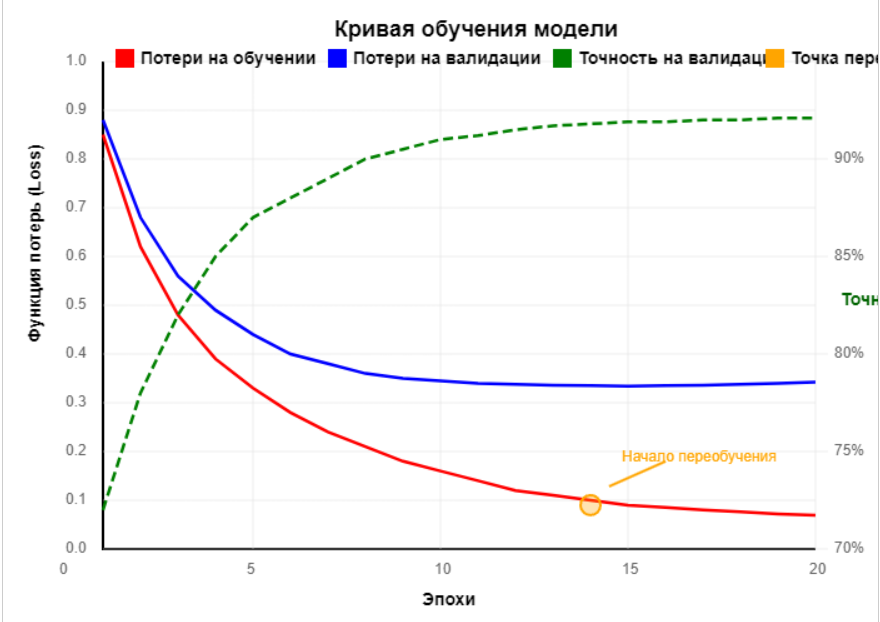
\includegraphics[width=0.8\textwidth]{figures/learning_curve.png}
\caption{Кривая обучения модели}
\label{fig:learning_curve}
\end{figure}

Результаты сравнения алгоритмов представлены в таблице~\ref{tab:results}.

\begin{table}[ht]
\caption{Сравнение алгоритмов классификации}
\centering
\begin{tabular}{|c|c|c|c|}
\hline
\texttt{Алгоритм} & \texttt{Точность (\%)} & \texttt{Время обучения (с)} & \texttt{F1-мера} \\
\hline
SVM & 94.2 & 2.3 & 0.94 \\
Логистическая регрессия & 92.1 & 1.1 & 0.92 \\
Градиентный бустинг & 96.7 & 5.8 & 0.96 \\
\hline
\end{tabular}
\label{tab:results}
\end{table}

\subsection{Анализ результатов}

Как видно из таблицы~\ref{tab:results}, алгоритм градиентного бустинга показывает наилучшую точность (96.7\%) и F1-меру (0.96), однако требует больше времени на обучение. Метод опорных векторов показывает хороший баланс между точностью и скоростью. Логистическая регрессия является самой быстрой, но уступает по качеству классификации \cite{attention}.

В коде из листинга \ref{code:python} реализовано обучение всех трех моделей с перекрестной проверкой. Переменная \texttt{C} в методе опорных векторов (см. формулу~\ref{eq:svm}) является гиперпараметром регуляризации.

\conclusion

В ходе выполнения работы были решены следующие задачи:
\begin{itemize}
    \item Проведен анализ методов классификации (SVM, логистическая регрессия, градиентный бустинг)
    \item Реализованы алгоритмы на языках Python и C++
    \item Выполнено сравнение эффективности алгоритмов на реальных данных
\end{itemize}

Экспериментально установлено, что градиентный бустинг показывает наилучшее качество классификации (96.7\%). Полученные результаты могут быть использованы в практических задачах классификации, включая медицинскую диагностику и анализ текстов \cite{classification_sound}.

\bibliographystyle{ugost2003}
\bibliography{thesis}

\end{document}